\begin{frame}{\small Global localisation: Το δεύτερο μεγαλύτερο πρόβλημα ρομποτικής κινητής βάσης}

  \vspace{-1cm}
  \noindent\makebox[0.6\linewidth][c]{%o
  \begin{minipage}{0.6\linewidth}

    \begin{figure}
      % GNUPLOT: LaTeX picture with Postscript
\begingroup
  \makeatletter
  \providecommand\color[2][]{%
    \GenericError{(gnuplot) \space\space\space\@spaces}{%
      Package color not loaded in conjunction with
      terminal option `colourtext'%
    }{See the gnuplot documentation for explanation.%
    }{Either use 'blacktext' in gnuplot or load the package
      color.sty in LaTeX.}%
    \renewcommand\color[2][]{}%
  }%
  \providecommand\includegraphics[2][]{%
    \GenericError{(gnuplot) \space\space\space\@spaces}{%
      Package graphicx or graphics not loaded%
    }{See the gnuplot documentation for explanation.%
    }{The gnuplot epslatex terminal needs graphicx.sty or graphics.sty.}%
    \renewcommand\includegraphics[2][]{}%
  }%
  \providecommand\rotatebox[2]{#2}%
  \@ifundefined{ifGPcolor}{%
    \newif\ifGPcolor
    \GPcolorfalse
  }{}%
  \@ifundefined{ifGPblacktext}{%
    \newif\ifGPblacktext
    \GPblacktexttrue
  }{}%
  % define a \g@addto@macro without @ in the name:
  \let\gplgaddtomacro\g@addto@macro
  % define empty templates for all commands taking text:
  \gdef\gplbacktext{}%
  \gdef\gplfronttext{}%
  \makeatother
  \ifGPblacktext
    % no textcolor at all
    \def\colorrgb#1{}%
    \def\colorgray#1{}%
  \else
    % gray or color?
    \ifGPcolor
      \def\colorrgb#1{\color[rgb]{#1}}%
      \def\colorgray#1{\color[gray]{#1}}%
      \expandafter\def\csname LTw\endcsname{\color{white}}%
      \expandafter\def\csname LTb\endcsname{\color{black}}%
      \expandafter\def\csname LTa\endcsname{\color{black}}%
      \expandafter\def\csname LT0\endcsname{\color[rgb]{1,0,0}}%
      \expandafter\def\csname LT1\endcsname{\color[rgb]{0,1,0}}%
      \expandafter\def\csname LT2\endcsname{\color[rgb]{0,0,1}}%
      \expandafter\def\csname LT3\endcsname{\color[rgb]{1,0,1}}%
      \expandafter\def\csname LT4\endcsname{\color[rgb]{0,1,1}}%
      \expandafter\def\csname LT5\endcsname{\color[rgb]{1,1,0}}%
      \expandafter\def\csname LT6\endcsname{\color[rgb]{0,0,0}}%
      \expandafter\def\csname LT7\endcsname{\color[rgb]{1,0.3,0}}%
      \expandafter\def\csname LT8\endcsname{\color[rgb]{0.5,0.5,0.5}}%
    \else
      % gray
      \def\colorrgb#1{\color{black}}%
      \def\colorgray#1{\color[gray]{#1}}%
      \expandafter\def\csname LTw\endcsname{\color{white}}%
      \expandafter\def\csname LTb\endcsname{\color{black}}%
      \expandafter\def\csname LTa\endcsname{\color{black}}%
      \expandafter\def\csname LT0\endcsname{\color{black}}%
      \expandafter\def\csname LT1\endcsname{\color{black}}%
      \expandafter\def\csname LT2\endcsname{\color{black}}%
      \expandafter\def\csname LT3\endcsname{\color{black}}%
      \expandafter\def\csname LT4\endcsname{\color{black}}%
      \expandafter\def\csname LT5\endcsname{\color{black}}%
      \expandafter\def\csname LT6\endcsname{\color{black}}%
      \expandafter\def\csname LT7\endcsname{\color{black}}%
      \expandafter\def\csname LT8\endcsname{\color{black}}%
    \fi
  \fi
    \setlength{\unitlength}{0.0500bp}%
    \ifx\gptboxheight\undefined%
      \newlength{\gptboxheight}%
      \newlength{\gptboxwidth}%
      \newsavebox{\gptboxtext}%
    \fi%
    \setlength{\fboxrule}{0.5pt}%
    \setlength{\fboxsep}{1pt}%
\begin{picture}(6000.00,6000.00)%
    \gplgaddtomacro\gplbacktext{%
    }%
    \gplgaddtomacro\gplfronttext{%
      \colorrgb{0.00,0.00,0.00}%
      \put(310,4777){\makebox(0,0)[l]{\strut{}Απαχθέν ρομπότ}}%
      \colorrgb{0.00,0.00,0.00}%
      \put(310,4457){\makebox(0,0)[l]{\strut{}Βάσει καθολικής αβεβαιότητας}}%
      \colorrgb{0.00,0.00,0.00}%
      \put(310,4137){\makebox(0,0)[l]{\strut{}Βάσει περιορισμένης αβεβαιότητας}}%
      \colorrgb{0.00,0.00,0.00}%
      \put(2120,3766){\makebox(0,0)[r]{\strut{}$19\%$}}%
      \put(1603,1878){\makebox(0,0)[r]{\strut{}$26\%$}}%
      \put(4455,2284){\makebox(0,0)[l]{\strut{}$55\%$}}%
    }%
    \put(0,0){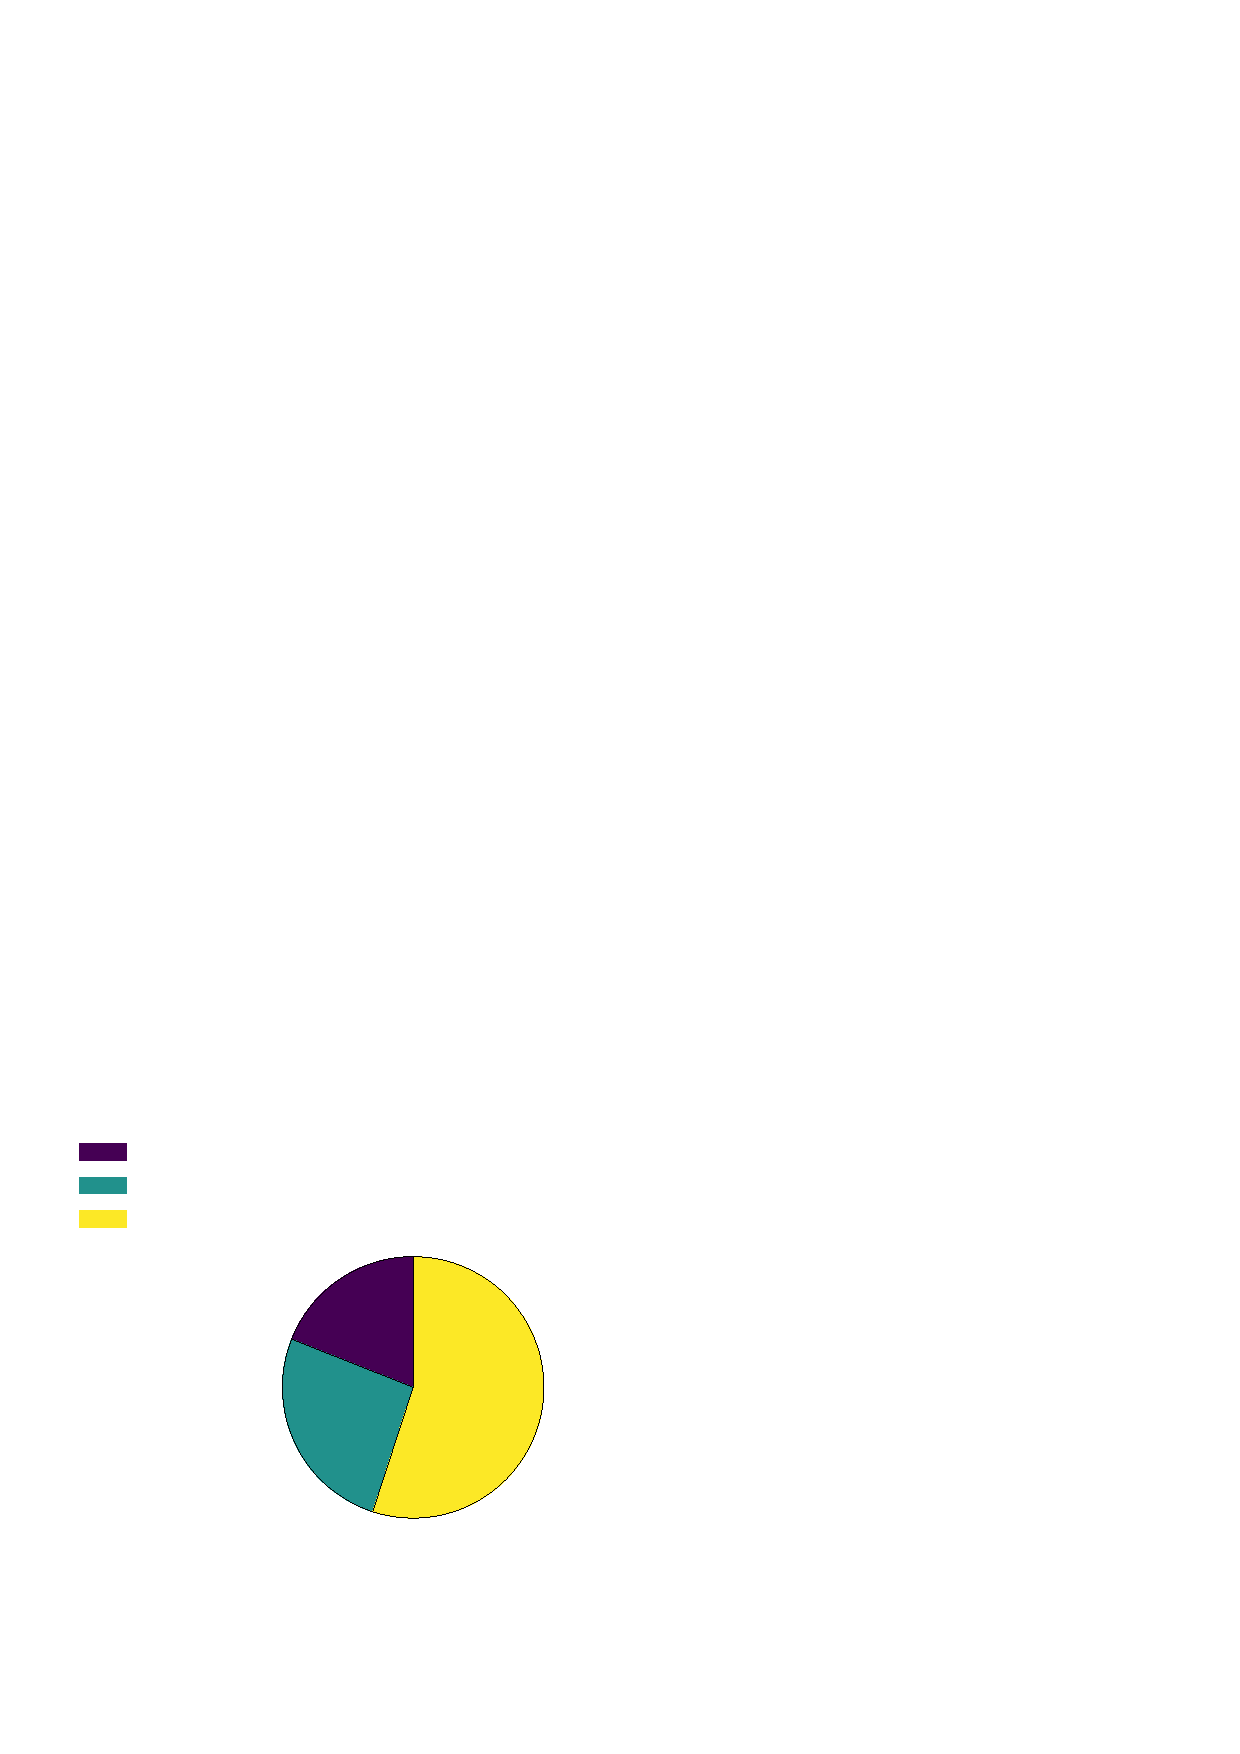
\includegraphics{./figures/parts/01/chapters/01/sections/01/localisation_problems_pie}}%
    \gplfronttext
  \end{picture}%
\endgroup

      \vspace{-1.5cm}
      \caption{\scriptsize Ποσοστά έρευνας στα προβλήματα εκτίμησης στάσης. Πηγή:
               Prabin Kumar Panigrahi and Sukant Kishoro Bisoy.  ``Localization
               strategies for autonomous mobile robots: A review",
               \textit{Journal of King Saud University - Computer and
               Information Sciences}, Mar. 2021.}
    \end{figure}

  \end{minipage}
  }
  \hfill
  \noindent\makebox[0.3\linewidth][c]{%
  \begin{minipage}{0.3\linewidth}
    \begin{figure}
      


\tikzset{every picture/.style={line width=0.75pt}} %set default line width to 0.75pt

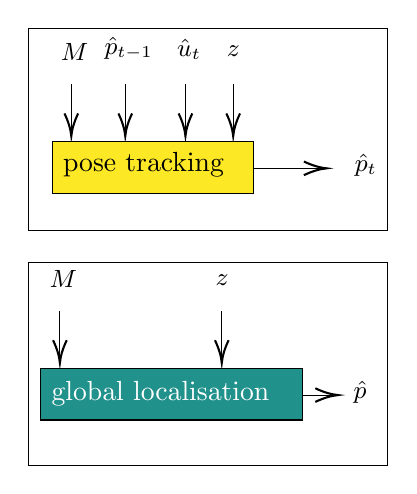
\begin{tikzpicture}[x=0.75pt,y=0.75pt,yscale=-1,xscale=1]
%uncomment if require: \path (0,300); %set diagram left start at 0, and has height of 300


%Straight Lines [id:da37620075399637964]
\draw    (130.25,28.5) -- (130.25,51.5) ;
\draw [shift={(130.25,53.5)}, rotate = 270] [color={rgb, 255:red, 0; green, 0; blue, 0 }  ][line width=0.75]    (10.93,-3.29) .. controls (6.95,-1.4) and (3.31,-0.3) .. (0,0) .. controls (3.31,0.3) and (6.95,1.4) .. (10.93,3.29)   ;
%Straight Lines [id:da8910828803681619]
\draw    (156.25,28.5) -- (156.25,51.5) ;
\draw [shift={(156.25,53.5)}, rotate = 270] [color={rgb, 255:red, 0; green, 0; blue, 0 }  ][line width=0.75]    (10.93,-3.29) .. controls (6.95,-1.4) and (3.31,-0.3) .. (0,0) .. controls (3.31,0.3) and (6.95,1.4) .. (10.93,3.29)   ;
%Straight Lines [id:da7026914270045463]
\draw    (185.25,28.5) -- (185.25,51.5) ;
\draw [shift={(185.25,53.5)}, rotate = 270] [color={rgb, 255:red, 0; green, 0; blue, 0 }  ][line width=0.75]    (10.93,-3.29) .. controls (6.95,-1.4) and (3.31,-0.3) .. (0,0) .. controls (3.31,0.3) and (6.95,1.4) .. (10.93,3.29)   ;
%Straight Lines [id:da07058947705205698]
\draw    (208.25,28.5) -- (208.25,51.5) ;
\draw [shift={(208.25,53.5)}, rotate = 270] [color={rgb, 255:red, 0; green, 0; blue, 0 }  ][line width=0.75]    (10.93,-3.29) .. controls (6.95,-1.4) and (3.31,-0.3) .. (0,0) .. controls (3.31,0.3) and (6.95,1.4) .. (10.93,3.29)   ;
%Straight Lines [id:da658480361580742]
\draw    (217.75,69) -- (251.25,69) ;
\draw [shift={(253.25,69)}, rotate = 180] [color={rgb, 255:red, 0; green, 0; blue, 0 }  ][line width=0.75]    (10.93,-3.29) .. controls (6.95,-1.4) and (3.31,-0.3) .. (0,0) .. controls (3.31,0.3) and (6.95,1.4) .. (10.93,3.29)   ;
%Straight Lines [id:da014317254825124026]
\draw    (124.75,137.75) -- (124.75,160.75) ;
\draw [shift={(124.75,162.75)}, rotate = 270] [color={rgb, 255:red, 0; green, 0; blue, 0 }  ][line width=0.75]    (10.93,-3.29) .. controls (6.95,-1.4) and (3.31,-0.3) .. (0,0) .. controls (3.31,0.3) and (6.95,1.4) .. (10.93,3.29)   ;
%Straight Lines [id:da6026375160663937]
\draw    (202.75,137.75) -- (202.75,160.75) ;
\draw [shift={(202.75,162.75)}, rotate = 270] [color={rgb, 255:red, 0; green, 0; blue, 0 }  ][line width=0.75]    (10.93,-3.29) .. controls (6.95,-1.4) and (3.31,-0.3) .. (0,0) .. controls (3.31,0.3) and (6.95,1.4) .. (10.93,3.29)   ;
%Straight Lines [id:da2508525371297663]
\draw    (241.25,178.25) -- (256.75,178.25) ;
\draw [shift={(258.75,178.25)}, rotate = 180] [color={rgb, 255:red, 0; green, 0; blue, 0 }  ][line width=0.75]    (10.93,-3.29) .. controls (6.95,-1.4) and (3.31,-0.3) .. (0,0) .. controls (3.31,0.3) and (6.95,1.4) .. (10.93,3.29)   ;
%Shape: Rectangle [id:dp5753636561604081]
\draw   (109.5,1.5) -- (282.75,1.5) -- (282.75,99) -- (109.5,99) -- cycle ;
%Shape: Rectangle [id:dp27272606446856584]
\draw   (109.5,114.5) -- (282.75,114.5) -- (282.75,212) -- (109.5,212) -- cycle ;

% Text Node
\draw  [fill={rgb, 255:red, 253; green, 232; blue, 38 }  ,fill opacity=1 ]  (121,56) -- (218,56) -- (218,81) -- (121,81) -- cycle  ;
\draw (125,60) node [anchor=north west][inner sep=0.75pt]   [align=left] {pose tracking};
% Text Node
\draw (124,7.75) node [anchor=north west][inner sep=0.75pt]   [align=left] {\small $\bm{M}$};
% Text Node
\draw (145,4.75) node [anchor=north west][inner sep=0.75pt]   [align=left] {\small $\hat{\bm{p}}_{t-1}$};
% Text Node
\draw (180,5.75) node [anchor=north west][inner sep=0.75pt]   [align=left] {\small $\hat{\bm{u}}_t$};
% Text Node
\draw (204,8.75) node [anchor=north west][inner sep=0.75pt]   [align=left] {\small $\bm{z}$};
% Text Node
\draw (265.6,61) node [anchor=north west][inner sep=0.75pt]   [align=left] {\small $\hat{\bm{p}}_{t}$};
% Text Node
\draw  [fill={rgb, 255:red, 33; green, 145; blue, 140 }  ,fill opacity=1 ]  (115.5,165.25) -- (241.5,165.25) -- (241.5,190.25) -- (115.5,190.25) -- cycle  ;
\draw (119.5,170.25) node [anchor=north west][inner sep=0.75pt] [color={rgb, 255:red, 255; green, 255; blue, 255 }  ,opacity=1 ]  [align=left] {global localisation};
% Text Node
\draw (265,170.25) node [anchor=north west][inner sep=0.75pt]  [align=left] {\small $\hat{\bm{p}}$};
% Text Node
\draw (118.5,117) node [anchor=north west][inner sep=0.75pt]   [align=left] {\small $\bm{M}$};
% Text Node
\draw (198.5,119) node [anchor=north west][inner sep=0.75pt]   [align=left] {\small $\bm{z}$};


\end{tikzpicture}

    \end{figure}
  \end{minipage}
    }

\note{\footnotesize
Κατά κύριο λόγο τα μεγάλα προβλήματα εκτίμησης στη ρομποτικής κινητής βάσης
διακρίνονται στα προβλήματα της παρατήρησης της στάσης ενός ρομπότ καθώς αυτό
κινείται, και στο πρόβλημα του global localisation, του προσδιορισμού δηλαδή
της στάσης του δεδομένων μόνο του χάρτη και μίας μέτρησης, όταν δεν υπάρχει
καμία πληροφορία για τη θέση και τον προσανατολισμό του ρομπότ.}

\end{frame}
